\section{Scaling, and a compilation cliff that bounds everything}
\label{sec:cliff}

The windowed formulation's central claim is that phase-register width
decouples from precision, and our measurements confirm it: window count and
per-circuit qubit width stay flat as precision rises
(Fig.~\ref{fig:scaling}).

\textbf{The binding constraint is elsewhere, and it is severe.} The
modular-arithmetic work register does not decouple, and in our reference
implementation it is compiled as a dense unitary. Table~\ref{tab:cliff}
gives the measured transpilation time: $0.14$\,s at 4 work qubits,
$0.38$\,s at 5, $2.1$\,s at 6, $42.2$\,s at 7, and a timeout at 8
($N\approx143$). The cliff is in Qiskit's generic unitary synthesis, not in
simulation, and it bites \emph{before a single shot is sampled}.

Two consequences follow, and they constrain every number in this article and
its companion. First, the reachable corpus is $N\le119$ in principle and
$N\in\{15,21\}$ in practice, since within the ceiling only those admit an odd
two-prime modulus with the even, non-trivial order that factor extraction
requires. Second, this is an artefact of our implementation choice, not of
the windowed method: a reversible ripple-carry construction
\cite{cuccaro2004} would replace the dense unitary and move the cliff. We
did not implement one, and we report the ceiling as an open limitation
rather than a property of the algorithm.

\begin{table}[htbp]
\centering\small
\caption{Measured transpilation time for the modular-multiplication
operator, before any sampling. The rise between 6 and 7 work qubits is a
factor of 20, and 8 work qubits does not complete within a $45$\,s timeout.
This is what confines the study to $N\in\{15,21\}$. From
\texttt{phase4\_transpile\_cliff.csv}.}
\label{tab:cliff}
\begin{tabular}{@{}rrrl@{}}
\toprule
$N$ & Work qubits & Transpile (s) & Status \\
\midrule
15  & 4 & 0.14  & completes \\
21  & 5 & 0.38  & completes \\
33  & 6 & 2.09  & completes \\
65  & 7 & 42.23 & completes \\
143 & 8 & $>45$ & \textbf{timeout} \\
\bottomrule
\end{tabular}
\end{table}

\begin{figure}[htbp]
\centering
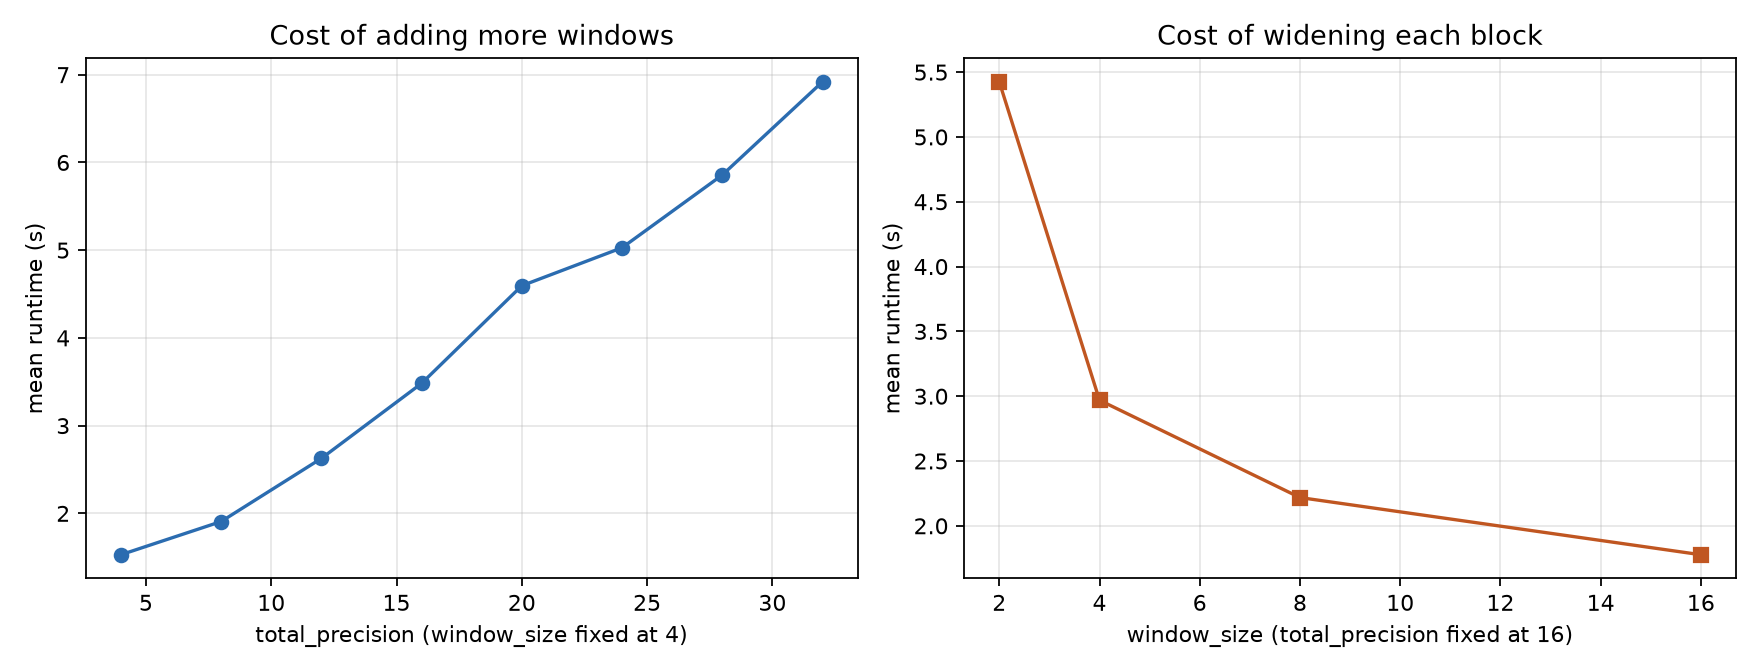
\includegraphics[width=0.86\linewidth]{../Data/failure_study/plots/scaling_decoupling.png}
\caption{\textbf{The decoupling claim holds on the phase side.} Window count
and per-circuit width stay flat as requested precision rises, which is the
saving the windowed formulation promises. The constraint that actually
bounds this study is on the work-register side and is in
Table~\ref{tab:cliff}. Rendered from \texttt{phase4\_scaling\_by\_*.csv}.}
\label{fig:scaling}
\end{figure}

% =====================================================================
